% ======================================================================
% Modelo de Decisión para Aprobación de Créditos y Segmentación de Riesgo
% Informe final — Licenciatura en Actuaría, Administración Actuarial
% Compilar: pdflatex informe.tex (x2) | biber/bibtex si se usa bibliografía
% ======================================================================
\documentclass[11pt,letterpaper]{article}

\usepackage[T1]{fontenc}
\usepackage[utf8]{inputenc}
\usepackage{lmodern}
\usepackage[spanish,mexico]{babel}
\usepackage[left=2.6cm,right=2.6cm,top=2.8cm,bottom=2.8cm]{geometry}
\usepackage{microtype}
\usepackage{amsmath,amssymb}
\usepackage{booktabs}
\usepackage{graphicx}
\usepackage{float}
\usepackage{array}
\usepackage{xcolor}
\usepackage{caption}
\usepackage{subcaption}
\usepackage{enumitem}
\usepackage[hidelinks]{hyperref}
\usepackage{fancyhdr}
\usepackage{lastpage}

\definecolor{azul}{RGB}{11,83,148}
\definecolor{azulfuerte}{RGB}{8,55,99}
\hypersetup{colorlinks=true,linkcolor=azul,urlcolor=azul,citecolor=azul}

\captionsetup{font=small,labelfont={bf,color=azulfuerte},skip=6pt}
\renewcommand{\arraystretch}{1.25}

\pagestyle{fancy}
\fancyhf{}
\fancyhead[L]{\small\color{azulfuerte}\textbf{Modelo de Decisión de Crédito}}
\fancyhead[R]{\small Administración Actuarial}
\fancyfoot[C]{\small Página \thepage\ de \pageref{LastPage}}

\begin{document}

% ----------------------------------------------------------------------
% PORTADA
% ----------------------------------------------------------------------
\begin{titlepage}
  \centering
  {\Large \textsc{Licenciatura en Actuaría}\par}
  {\large Facultad de Estudios Superiores Acatlán, UNAM\par}
  {\large Asignatura: Administración Actuarial\par}
  \vspace{1.2cm}
  {\color{azulfuerte}\rule{\linewidth}{1.2pt}\par}
  \vspace{0.8cm}
  {\Huge\bfseries\color{azulfuerte} Modelo de Decisión para la\\[2pt]
   Aprobación de Créditos y\\[2pt] Segmentación de Riesgo\par}
  \vspace{0.8cm}
  {\color{azulfuerte}\rule{\linewidth}{1.2pt}\par}
  \vspace{1.2cm}
  {\large\bfseries Informe técnico final\par}
  \vspace{0.4cm}
  {\large Autor: \textbf{Orlando Barcena Romero}\par}
  \vspace{1.5cm}
  \begin{minipage}{0.72\linewidth}
    \small
    \textit{Resumen ejecutivo:} se desarrolla un modelo estadístico de
    aprobación crediticia que acepta únicamente 25\% de las solicitudes
    recibidas y clasifica a los aprobados en segmentos de riesgo
    \textit{Bueno} y \textit{Malo}. Con regresión logística sobre variables de
    solicitud y validación en muestra de test, el modelo alcanza un AUROC de
    \textbf{0.746}, excluye de la cartera al \textbf{84\%} de los préstamos
    incumplidos y reduce un tercio la morosidad de la cartera frente al
    modelo de reglas de la práctica tradicional de la asignatura.
  \end{minipage}
  \vfill
  {\large Ciclo escolar 2025--2026\par}
\end{titlepage}

% ----------------------------------------------------------------------
% TABLA DE CONTENIDO
% ----------------------------------------------------------------------
\tableofcontents
\newpage

% ----------------------------------------------------------------------
% 1. INTRODUCCIÓN
% ----------------------------------------------------------------------
\section{Introducción y planteamiento del problema}

El otorgamiento de crédito es la actividad central de instituciones financieras
y aseguradoras de cartera, y su rentabilidad depende de un equilibrio
fundamental: \emph{aprobar más solicitudes implica mayor volumen de negocio,
pero también mayor exposición a incumplimiento}. La función actuarial participa
en este equilibrio mediante la \textbf{medición y administración del riesgo de
crédito}, definiendo políticas de originación basadas en la solvencia del
solicitante.

En el presente proyecto se plantea un escenario operativo con una restricción
explícita de política:

\begin{quote}
\textit{La institución solo puede aprobar el \textbf{25\%} de las solicitudes
de crédito que recibe, y requiere clasificar a los aceptados en dos segmentos:
\textbf{Buenos} (riesgo bajo, tratamiento preferente) y \textbf{Malos} (riesgo
controlado, seguimiento especial).}
\end{quote}

Esta restricción es común en entornos de \emph{capacidad de fondeo limitada} o
de \emph{apetito de riesgo} definido por la alta dirección. El problema se
descompone en dos tareas complementarias:

\begin{enumerate}[label=\textbf{T\arabic*.},leftmargin=1.6em]
  \item \textbf{Selección.} Elegir exactamente al 25\% de solicitantes con el
        menor riesgo de incumplimiento.
  \item \textbf{Segmentación.} Dentro de los aprobados, separar a los clientes
        de perfil \emph{Bueno} de los de perfil \emph{Malo} para administrar
        diferencialmente la cartera (tasas, límites, monitoreo y provisiones).
\end{enumerate}

El trabajo se desarrolla sobre datos públicos de préstamos personales de
Lending Club, y constituye una evolución profesional del ejercicio de reglas
de decisión realizado en clase: se conserva el objetivo de negocio, pero la
selección se funda en un \textbf{modelo estadístico validado} en lugar de
criterios heurísticos.

La estructura del informe es la siguiente: la Sección 2 presenta el marco
teórico del riesgo de crédito y de las métricas de capacidad discriminatoria;
la Sección 3 describe los datos; la Sección 4 detalla la metodología, incluida
la construcción de umbrales operativos; la Sección 5 reporta los resultados;
la Sección 6 discute sus implicaciones y limitaciones; y la Sección 7 cierra
con conclusiones y trabajo futuro.

% ----------------------------------------------------------------------
% 2. MARCO TEÓRICO
% ----------------------------------------------------------------------
\section{Marco teórico}

\subsection{Riesgo de crédito y probabilidad de incumplimiento}

El riesgo de crédito es la probabilidad de que un deudor no cumpla con sus
obligaciones de pago conforme a lo pactado \cite{bcbs2005,thomas2002}. La
herramienta actuarial estándar para administrarlo es el \textbf{modelo de
scoring}, que asigna a cada solicitante un puntaje proporcional a su riesgo
estimado \cite{anderson2007}. En la práctica se identifican tres etapas:
\emph{originación} (decisiones de aceptación), \emph{comportamiento}
(gestión de la cartera en vigor) y \emph{cobranza}.

\subsection{Modelo de regresión logística}

Sea $Y \in \{0,1\}$ el estado del préstamo ($Y=1$ si es \emph{malo}) y
$\mathbf{x}$ el vector de características del solicitante. El modelo de
regresión logística postula

\begin{equation}
  P(Y=1 \mid \mathbf{x}) = \frac{1}{1 + e^{-(\beta_0 + \boldsymbol{\beta}^\top \mathbf{x})}},
  \label{eq:logit}
\end{equation}

estimándose $\beta_0,\boldsymbol{\beta}$ por máxima verosimilitud. Su
popularidad en la industria se debe a que es \emph{calibrado} (las
probabilidades estimadas son directamente utilizables), \emph{interpretable}
(coeficientes con signo económico claro) y \emph{estable} frente a muestras
pequeñas, además de servir de base para \emph{scorecards} cuadráticos
\cite{anderson2007}.

\subsection{Scorecard crediticio}

Un scorecard transforma la probabilidad del modelo en una escala aditiva de
puntos comparable al puntaje FICO:

\begin{equation}
  \text{Score} = \text{offset} - \text{factor} \times \ln\!\left(\frac{p}{1-p}\right),
  \label{eq:score}
\end{equation}

donde $p/(1-p)$ es el \emph{odds} de incumplimiento. El parámetro
$\text{factor}$ fija cuántos puntos valen dichas probabilidades ($20$ puntos
por duplicar el odds es la convención de la industria) y $\text{offset}$ ancla
la escala a un punto de referencia. Así, \textbf{mayor puntaje implica menor
riesgo} y los umbrales de decisión se expresan en puntos, lenguaje con el que
operan las áreas de crédito y cumplimiento.

\subsection{Métricas de capacidad discriminatoria}

La capacidad del score para separar buenos de malos se mide con:

\begin{itemize}[leftmargin=1.6em]
  \item \textbf{AUROC} (área bajo la curva ROC): probabilidad de que el modelo
        asigne mayor riesgo a un incumplido elegido al azar que a un
        cumplido \cite{hanley1982}. Va de 0.5 (azar) a 1 (separación perfecta);
        en aplicaciones crediticias valores entre 0.70 y 0.80 se consideran
        buenos \cite{siddiqi2006}.
  \item \textbf{GINI}: transformación lineal del AUROC, $\text{GINI} =
        2\,\text{AUROC} - 1$; se interpreta como la proporción de la
        distribución de malos capturada por encima del azar.
  \item \textbf{KS} (Kolmogorov--Smirnov): máxima distancia vertical entre las
        distribuciones acumuladas de buenos y malos ordenadas por el score;
        mide la separación alcanzada en el punto más favorable del ordenamiento.
\end{itemize}

Adicionalmente se reportan \textbf{métricas de negocio} que conectan el modelo
con la restricción operativa: tasa de aprobación, tasa de incumplimiento en la
cartera aprobada y en la rechazada, y \emph{captura de malos} (proporción de
incumplidos excluidos de la cartera).

% ----------------------------------------------------------------------
% 3. DATOS
% ----------------------------------------------------------------------
\section{Datos}

\subsection{Fuente y alcance}

La información proviene de la base pública de préstamos personales de
\textbf{Lending Club}, originados entre 2007 y 2015. El archivo
\emph{LCDataDictionary} documenta 80 variables; la base de trabajo contiene
\emph{42} variables y \textbf{292{,}849} solicitudes. Para el análisis se
conservan las variables de la solicitud (identidad del solicitante y de la
operación) y las de desempeño del préstamo (pagos recibidos), que permiten
construir la variable objetivo.

\subsection{Preprocesamiento}

El pipeline de preparación de datos (\texttt{00\_preprocess.py}) realiza:

\begin{enumerate}
  \item \textbf{Parseo de fechas} (emisión y origen del historial crediticio),
        independiente del \emph{locale} del sistema, para derivar la
        \emph{antigüedad del historial} en meses.
  \item \textbf{Depuración de amplitudes}: recorte de valores extremos no
        plausibles (DTI, tasas, utilización de líneas) y conversión de tipos.
  \item \textbf{Ingeniería de variables}: codificación ordinal de
        \texttt{grade} y \texttt{emp\_length}, logaritmos de montos e
        ingresos, y banderas de información faltante.
  \item \textbf{Definición del objetivo}: un préstamo es \emph{malo} si la
        \textbf{recuperación de principal} ($\text{total\_rec\_prncp} /
        \text{funded\_amnt}$) es inferior a \textbf{70\%};
        \emph{bueno} en caso contrario.
\end{enumerate}

Los valores faltantes se imputan con la \textbf{mediana} dentro del pipeline de
modelado, ajustada únicamente sobre la muestra de entrenamiento, lo que evita
fuga de información hacia la muestra de validación.

\subsection{Estadística descriptiva}

La Tabla~\ref{tab:perfil} compara los perfiles de buenos y malos préstamos, y
la Figura~\ref{fig:grade} muestra la tasa de incumplimiento observada por
calificación crediticia.

\begin{table}[H]
  \centering
  \caption{Perfil comparativo de buenos y malos préstamos}
  \label{tab:perfil}
  \small
  \begin{tabular}{lrr}
    \toprule
    Variable (promedio) & Bueno ($n=81{,}834$) & Malo ($n=211{,}015$) \\
    \midrule
    Monto solicitado (USD)          & 13{,}246  & 15{,}342 \\
    Tasa de interés (\% anual)      & 13.24     & 13.26 \\
    Ingreso anual (USD)             & 73{,}543  & 75{,}558 \\
    Relación deuda--ingreso (\%)    & 16.17     & 18.89 \\
    Morosidades en 2 años           & 0.24      & 0.34 \\
    Meses desde última morosidad    & 35.21     & 33.73 \\
    Antigüedad del historial (m)    & 184.6     & 200.7 \\
    Utilización de líneas (\%)      & 53.8      & 55.6 \\
    Recuperación de principal (\%)  & 97.3      & 20.8 \\
    \bottomrule
  \end{tabular}
\end{table}

\begin{figure}[H]
  \centering
  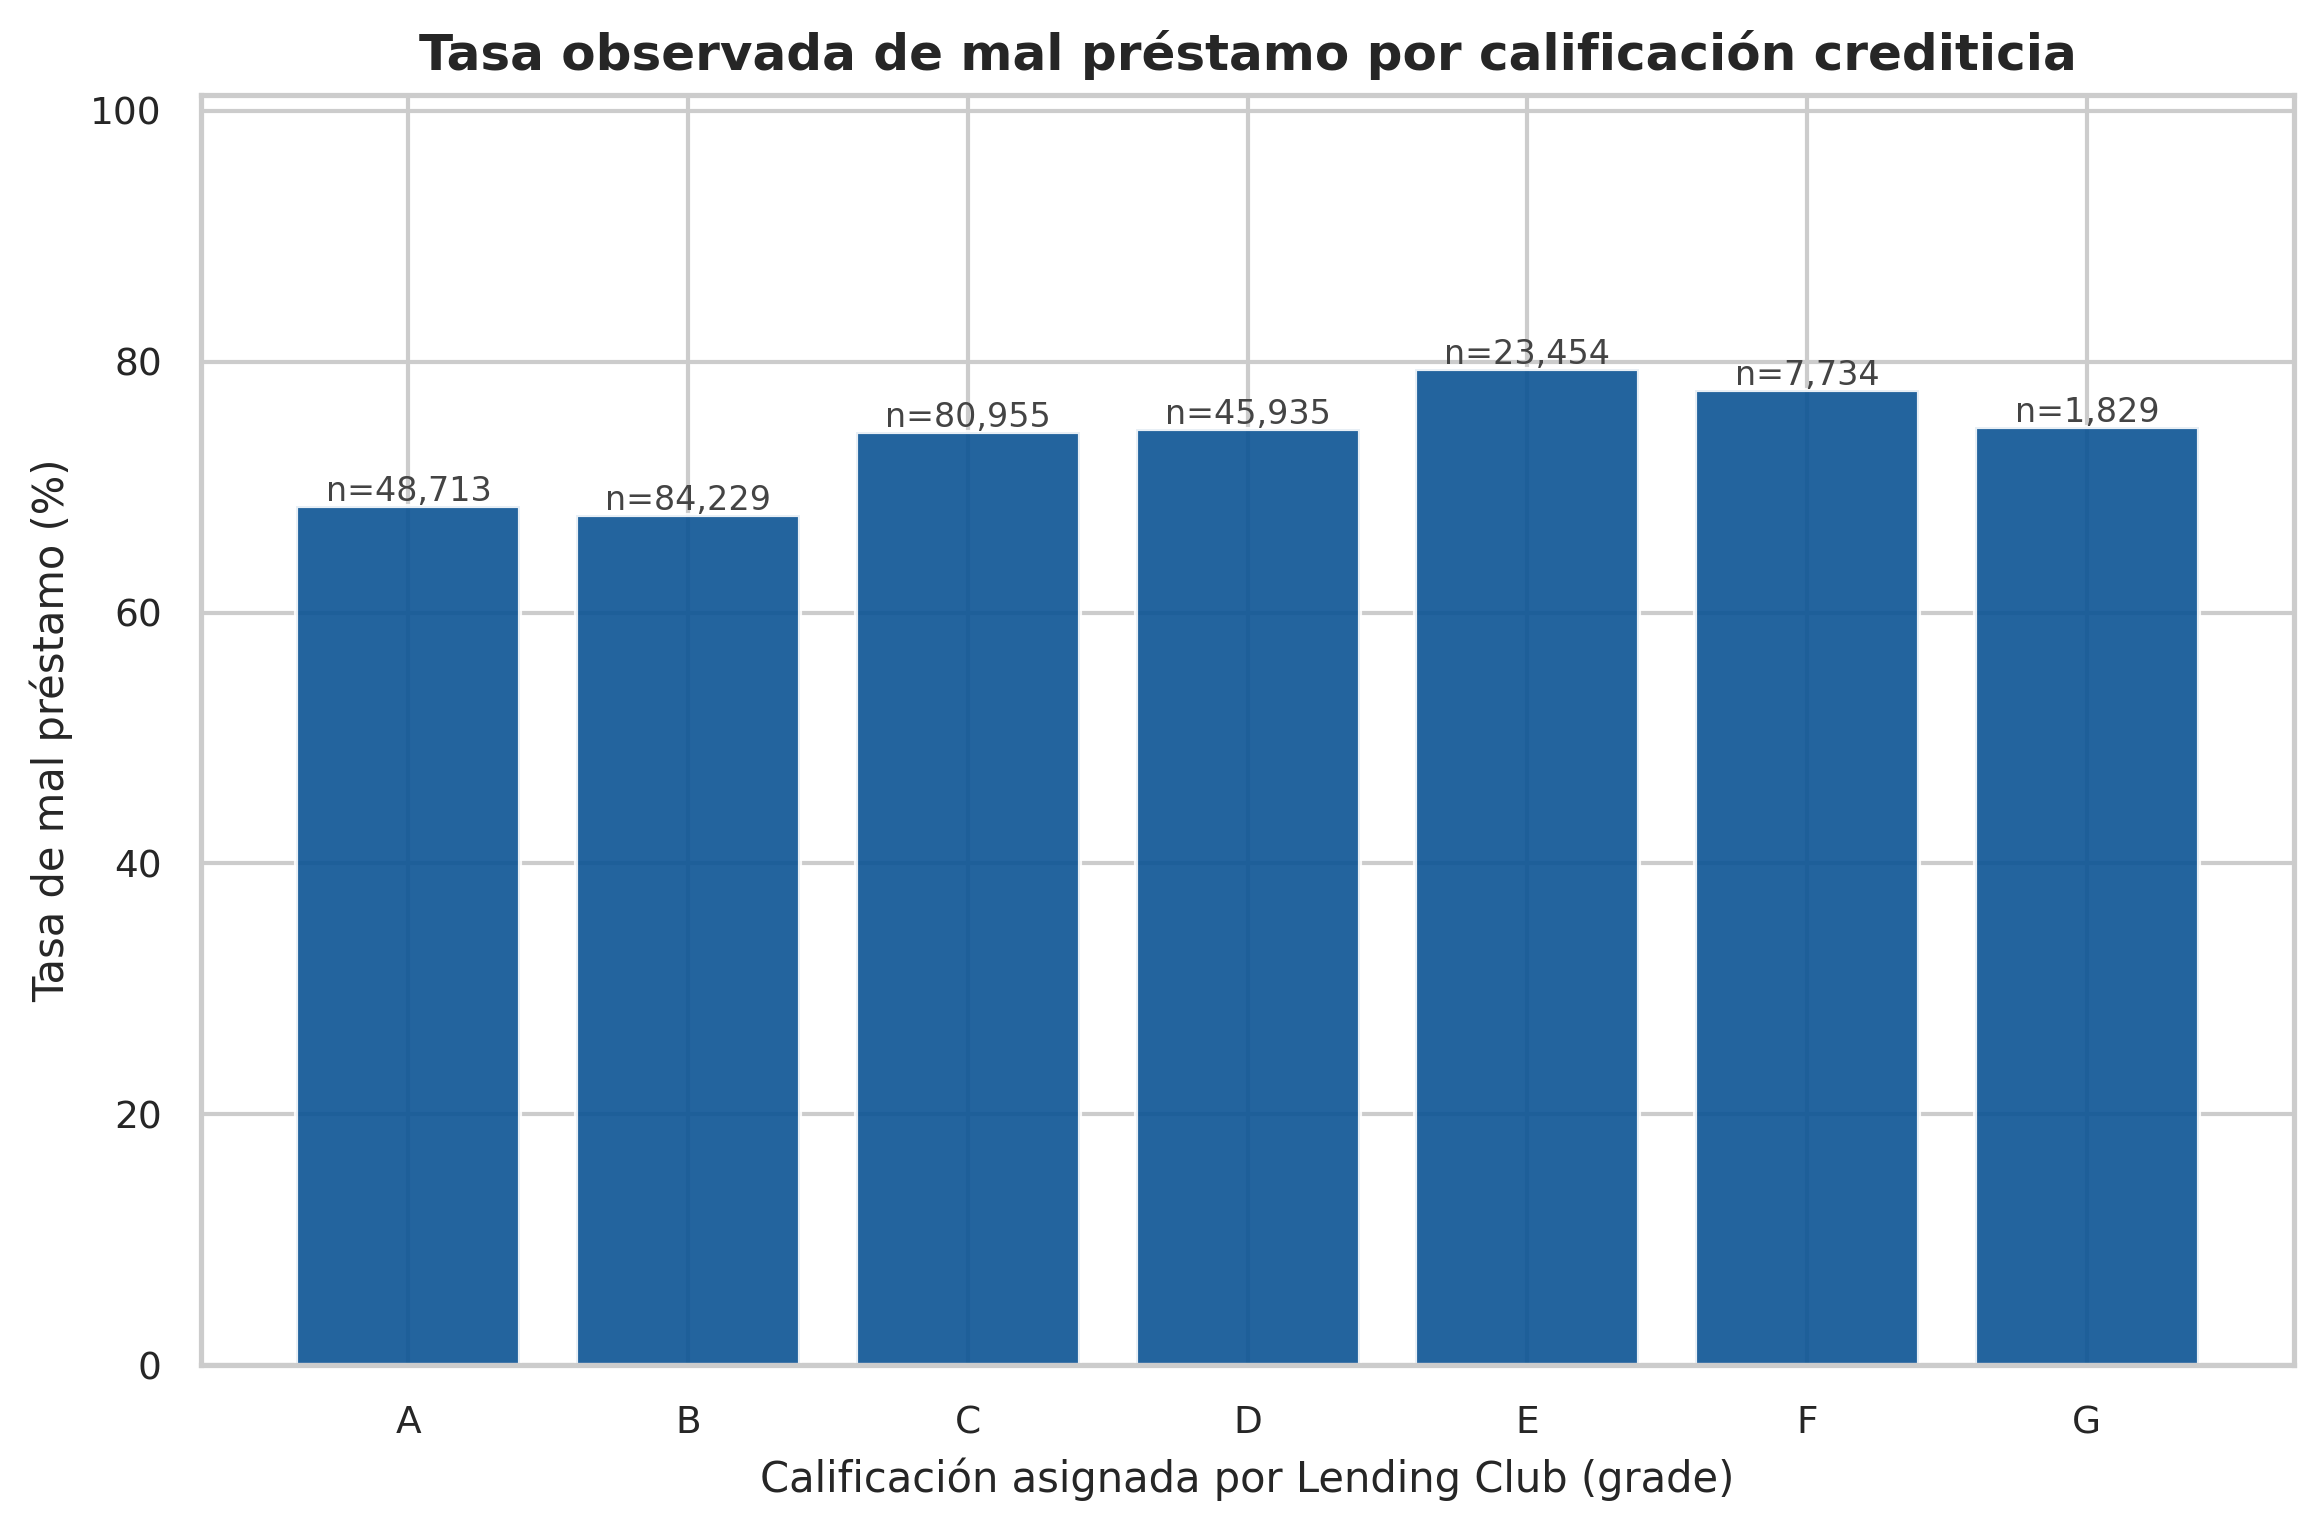
\includegraphics[width=0.72\linewidth]{figuras/eda_bad_rate_by_grade.png}
  \caption{Tasa de mal préstamo por calificación crediticia. La tasa crece
  monótonamente de \texttt{A} a \texttt{G}, confirmando que la calificación
  del originador resume riesgo, aunque con traslape suficiente para que un
  modelo estadístico agregue valor.}
  \label{fig:grade}
\end{figure}

La tasa global de préstamos malos es de \textbf{72.1\%}. Este valor es alto
porque la base incluye operaciones de la crisis 2008--2009 y el criterio de
recuperación es exigente; no representa la morosidad promedio de la industria,
sino la definición operativa de este ejercicio.

% ----------------------------------------------------------------------
% 4. METODOLOGÍA
% ----------------------------------------------------------------------
\section{Metodología}

\subsection{Diseño experimental}

Se divide la base en entrenamiento (70\%) y test (30\%) con estratificación
por la variable objetivo y semilla fija ($42$), de modo que los umbrales
operativos se calibran exclusivamente con información de entrenamiento y se
evalúan en muestra no vista. La proporción de malos es idéntica en ambas
muestras (72.1\%).

\subsection{Variables del modelo (sin leakage)}

Solo se utilizan variables \textbf{disponibles al momento de la solicitud};
quedan excluidas todas las variables de resultado (pagos recibidos,
recuperaciones, saldos). La matriz final contiene \textbf{44} variables:
22 numéricas (monto, tasa, DTI, morosidades, antigüedad del historial,
utilización de líneas, banderas de faltante, etc.) y 22 dummies derivadas de
\texttt{home\_ownership}, \texttt{verification\_status} y \texttt{purpose}.
Todas se estandarizan dentro del pipeline.

\subsection{Estimación y scorecard}

Se estima la regresión logística \eqref{eq:logit} y se transforma al scorecard
\eqref{eq:score} con $\text{factor} = 20/\ln 2 \approx 28.85$ (20 puntos por
duplicación de odds) y un punto de anclaje tal que el umbral de aprobación
coincida con $\text{Score} = 600$.

\subsection{Umbrales operativos}

Sobre la muestra de entrenamiento:

\begin{enumerate}
  \item \textbf{Aprobación:} $\text{p}^* = Q_{0.25}(\hat{p}_{train})$,
        el cuantil 25\% de las probabilidades de incumplimiento estimadas.
        Aprobar a los 25\% de solicitantes con $\hat{p} \leq p^*$ equivale al
        punto de corte $\text{Score} \geq 600$.
  \item \textbf{Sub-segmentación:} entre los aprobados, el segmento
        \emph{Bueno} corresponde a los puntajes por encima de la mediana del
        grupo (Score $\geq 613$) y el \emph{Malo} al resto.
\end{enumerate}

\subsection{Sistemas de referencia: modelo de reglas}

Se reproduce el modelo de reglas del ejercicio de clase como referencia:
\textbf{condición principal} (meses desde la última morosidad $\geq 30$ o sin
registro) más el cumplimiento de al menos 3 de 4 condiciones secundarias
(DTI $\leq 22$; \texttt{grade} = A; sin morosidades en 2 años; recuperación
$\geq 70\%$). Se reportan dos variantes:

\begin{itemize}
  \item \textbf{Con recuperación} (variante del ejercicio): incluye la regla
        de desempeño, lo que constituye \emph{leakage} —usa una variable de
        resultado para decidir sobre ese mismo resultado— y sobreestima sus
        métricas.
  \item \textbf{Sin recuperación}: variante operable en la práctica.
\end{itemize}

% ----------------------------------------------------------------------
% 5. RESULTADOS
% ----------------------------------------------------------------------
\section{Resultados}

\subsection{Capacidad discriminatoria}

La Tabla~\ref{tab:disc} resume las métricas en ambas muestras. El modelo
generaliza sin sobreajuste: las métricas son prácticamente idénticas en train
y test.

\begin{table}[H]
  \centering
  \caption{Métricas de discriminación del scorecard}
  \label{tab:disc}
  \small
  \begin{tabular}{lccc}
    \toprule
    Muestra & AUROC & GINI & KS \\
    \midrule
    Entrenamiento ($n=204{,}994$) & 0.7462 & 0.4924 & 0.3702 \\
    Test ($n=87{,}855$)           & 0.7462 & 0.4924 & 0.3700 \\
    \bottomrule
  \end{tabular}
\end{table}

\begin{figure}[H]
  \centering
  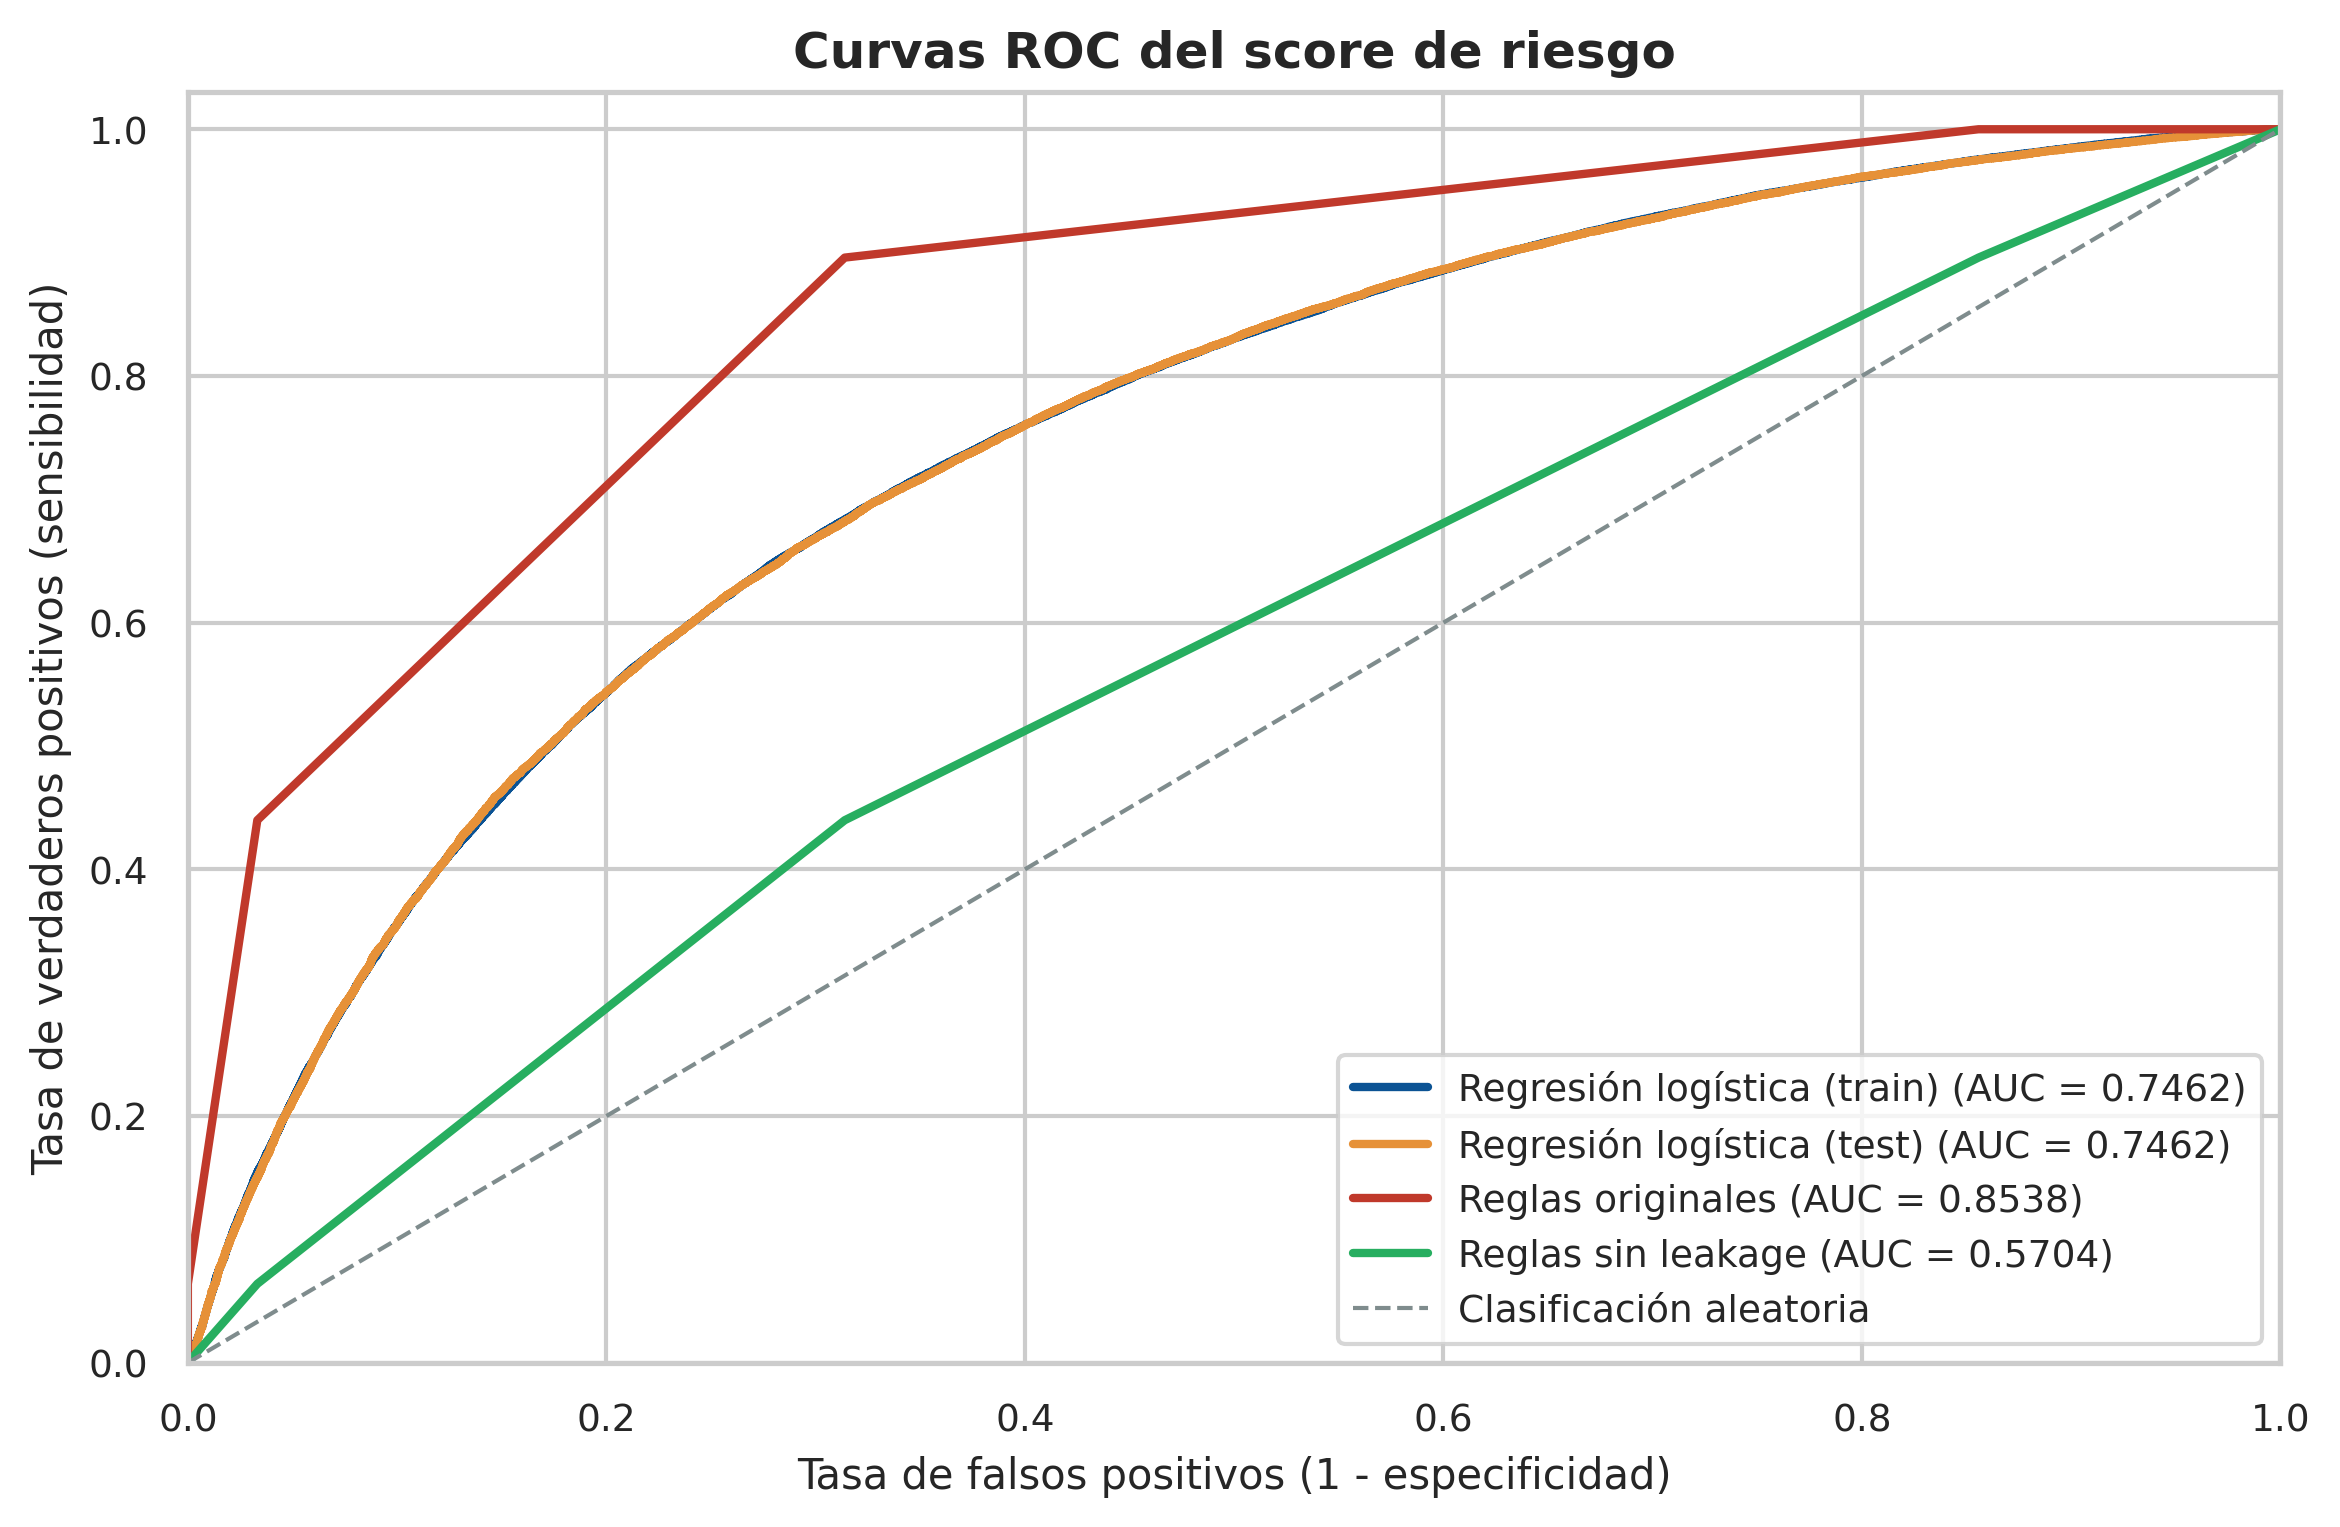
\includegraphics[width=0.80\linewidth]{figuras/model_roc.png}
  \caption{Curvas ROC del modelo logístico (train y test) y de las reglas del
  ejercicio. La variante ``con recuperación'' infla artificialmente el AUC por
  leakage; la comparación honesta es contra la variante operable (AUC 0.57).}
  \label{fig:roc}
\end{figure}

La Figura~\ref{fig:dist} muestra que los puntajes de buenos y malos se
superponen parcialmente con centros separados, y que la política de aprobación
(Score $\geq 600$) concentra a los buenos.

\begin{figure}[H]
  \centering
  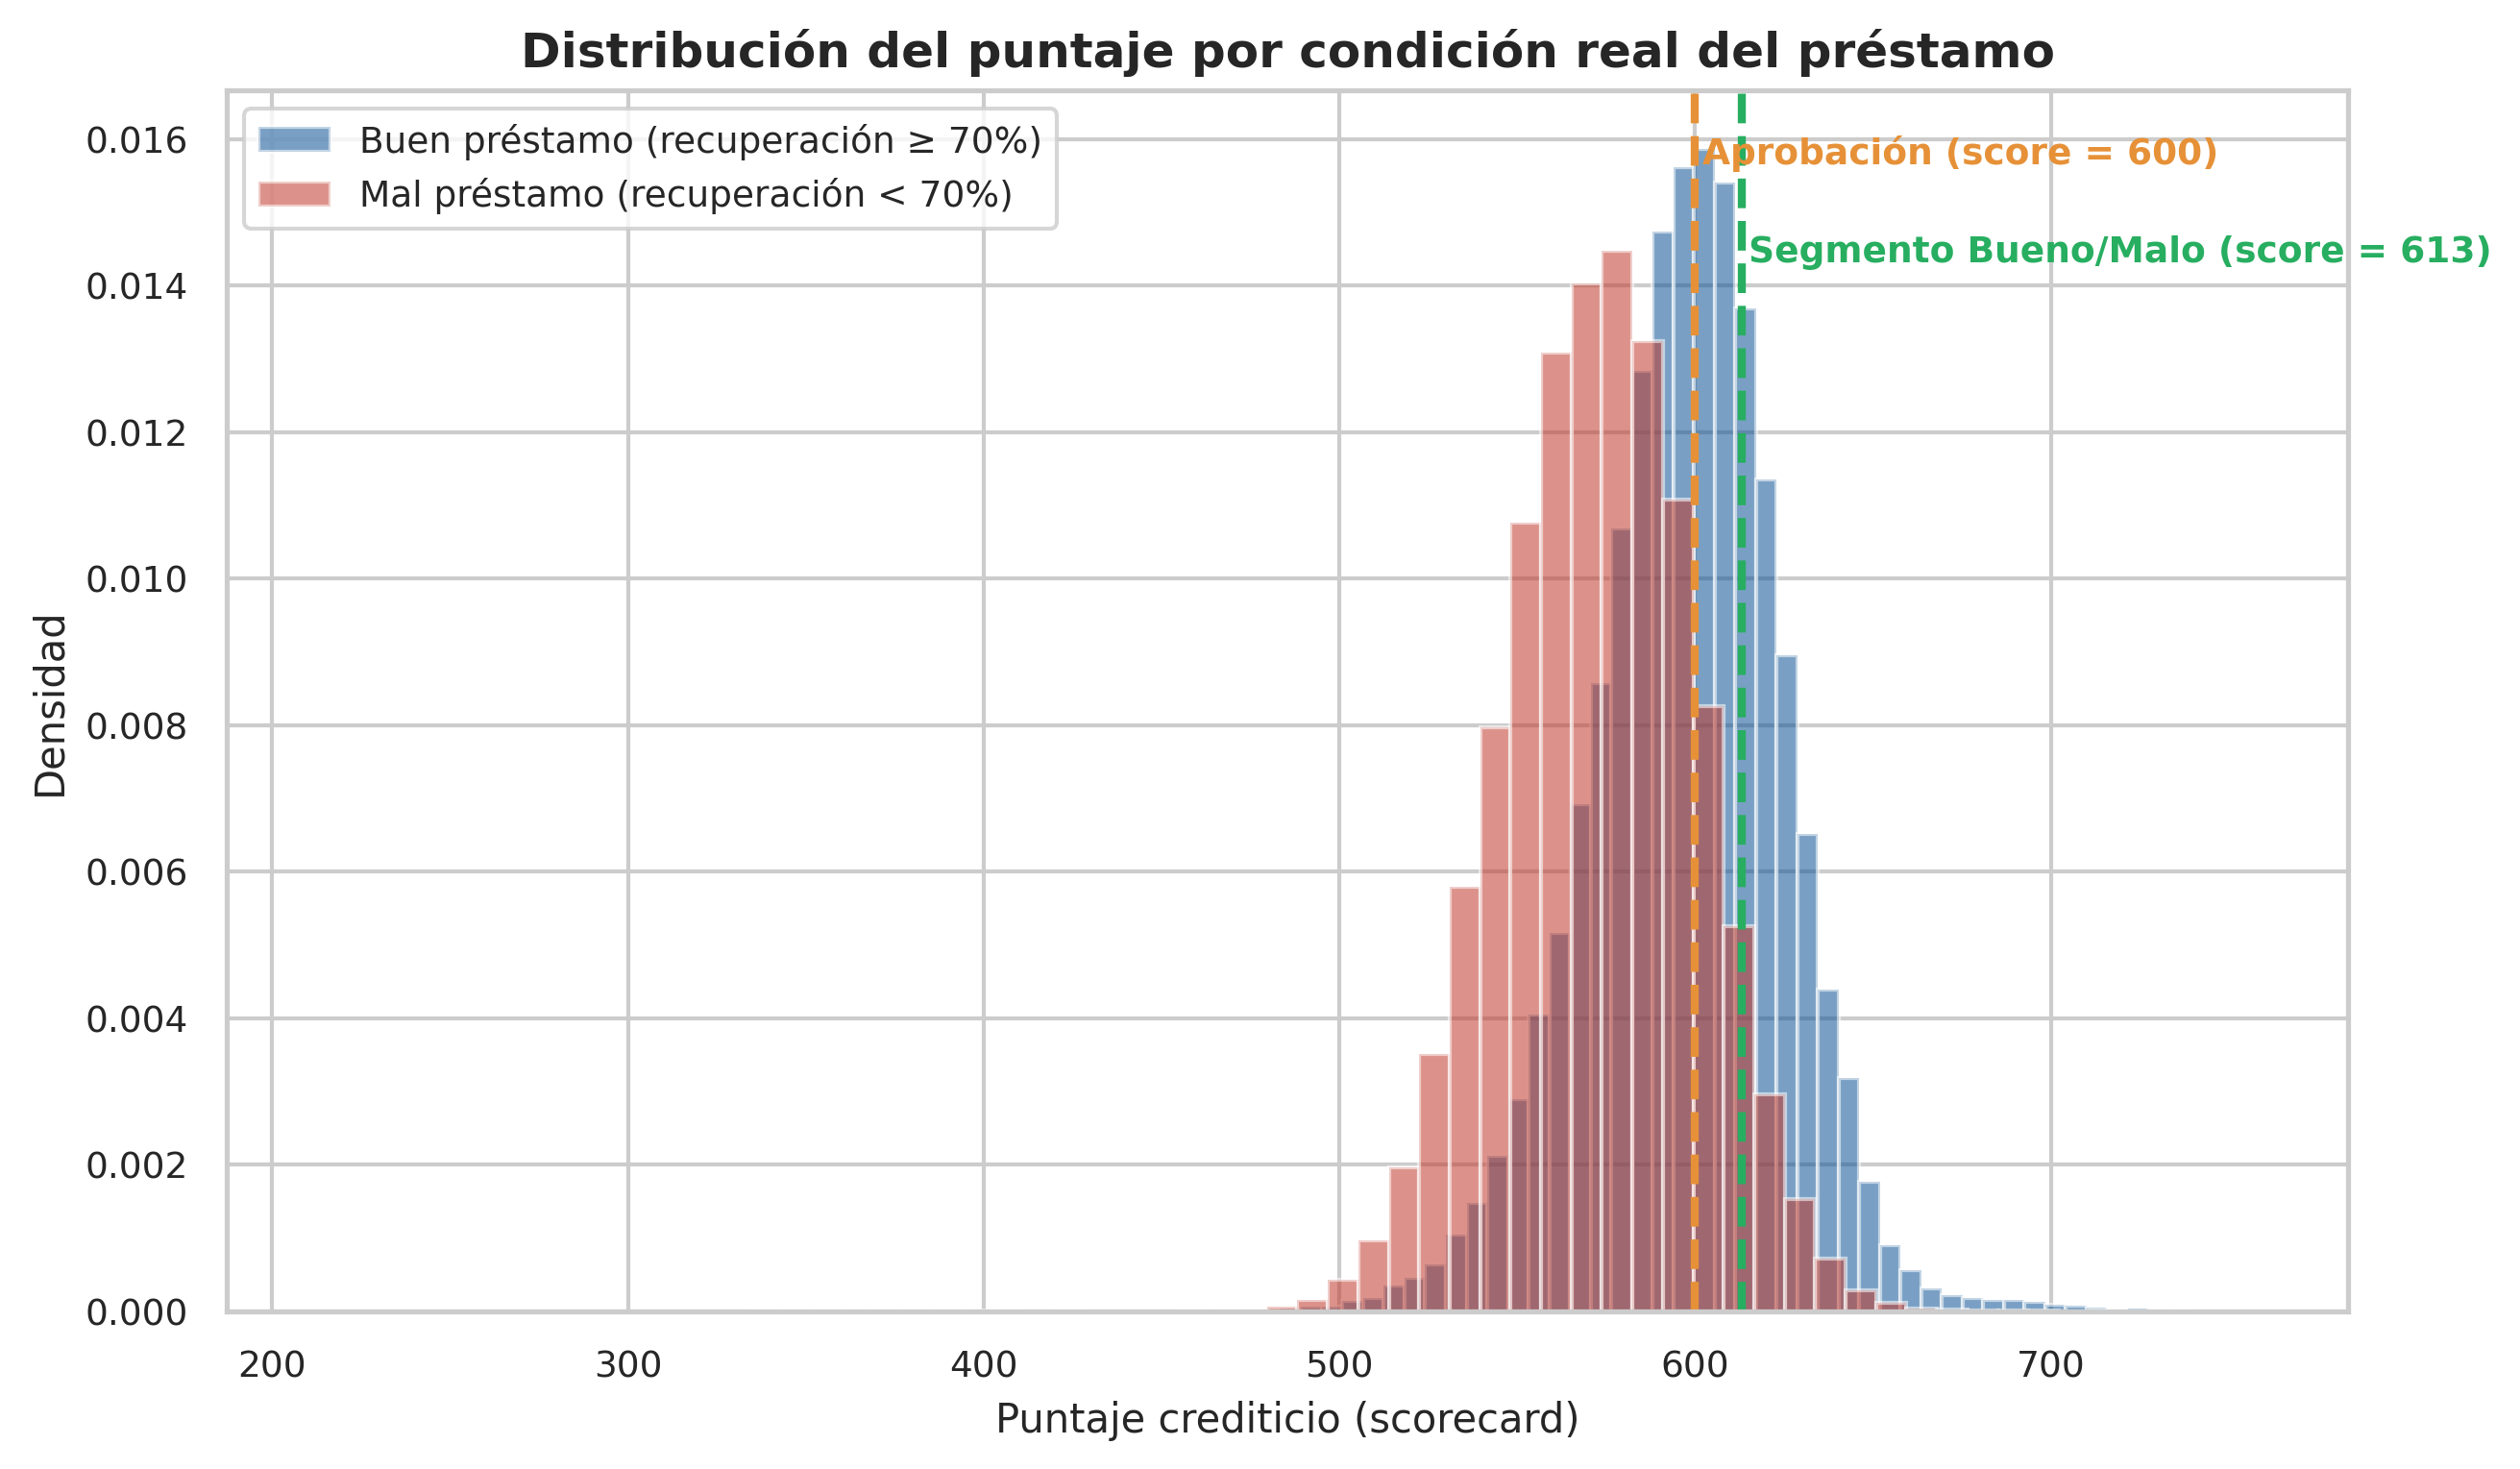
\includegraphics[width=0.78\linewidth]{figuras/model_score_distribution.png}
  \caption{Distribución del puntaje por condición real del préstamo y ubicación
  de los umbrales de decisión.}
  \label{fig:dist}
\end{figure}

\subsection{Política de aprobación al 25\%}

La Tabla~\ref{tab:aprob} presenta las métricas de negocio en la muestra de
test. La tasa de aprobación efectiva es \textbf{24.88\%} (objetivo 25\%); la
cartera aprobada concentra una tasa de malos (45.8\%) claramente inferior a la
población (72.1\%) y a la de los rechazados (80.8\%).

\begin{table}[H]
  \centering
  \caption{Métricas de la política de aprobación en la muestra de test}
  \label{tab:aprob}
  \small
  \begin{tabular}{lcc}
    \toprule
    Indicador & Valor \\
    \midrule
    Solicitudes evaluadas & 87{,}855 \\
    Tasa de aprobación & 24.88\% \\
    Tasa de malos en aprobados & 45.8\% \\
    Tasa de malos en rechazados & 80.8\% \\
    Captura de malos (excluidos de cartera) & 84.2\% \\
    Tasa de malos del segmento \emph{Bueno} ($n=11{,}091$) & 37.5\% \\
    Tasa de malos del segmento \emph{Malo} ($n=10{,}766$) & 54.3\% \\
    \bottomrule
  \end{tabular}
\end{table}

\begin{figure}[H]
  \centering
  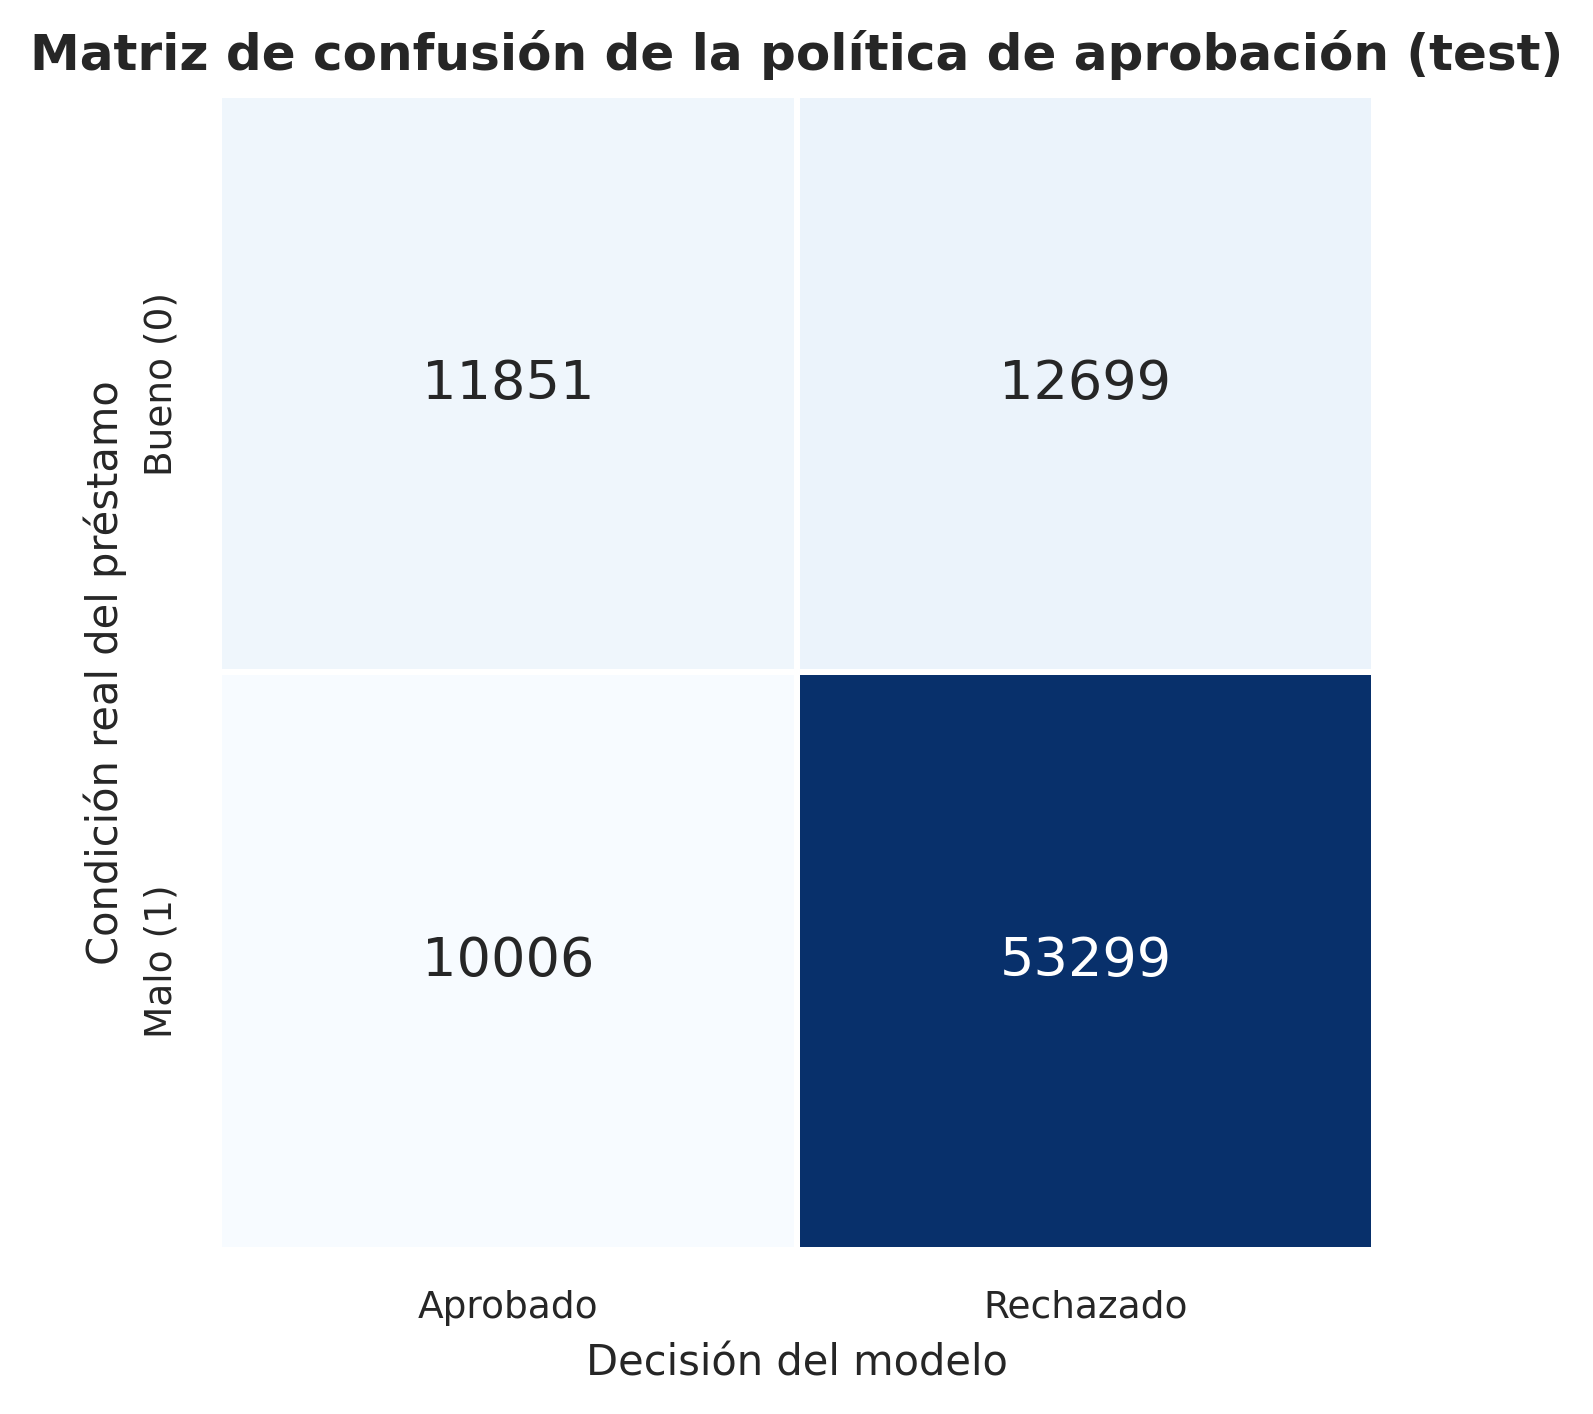
\includegraphics[width=0.80\linewidth]{figuras/model_confusion_matrix.png}
  \caption{Matriz de confusión de la política de aprobación en test.}
  \label{fig:cm}
\end{figure}

\begin{figure}[H]
  \centering
  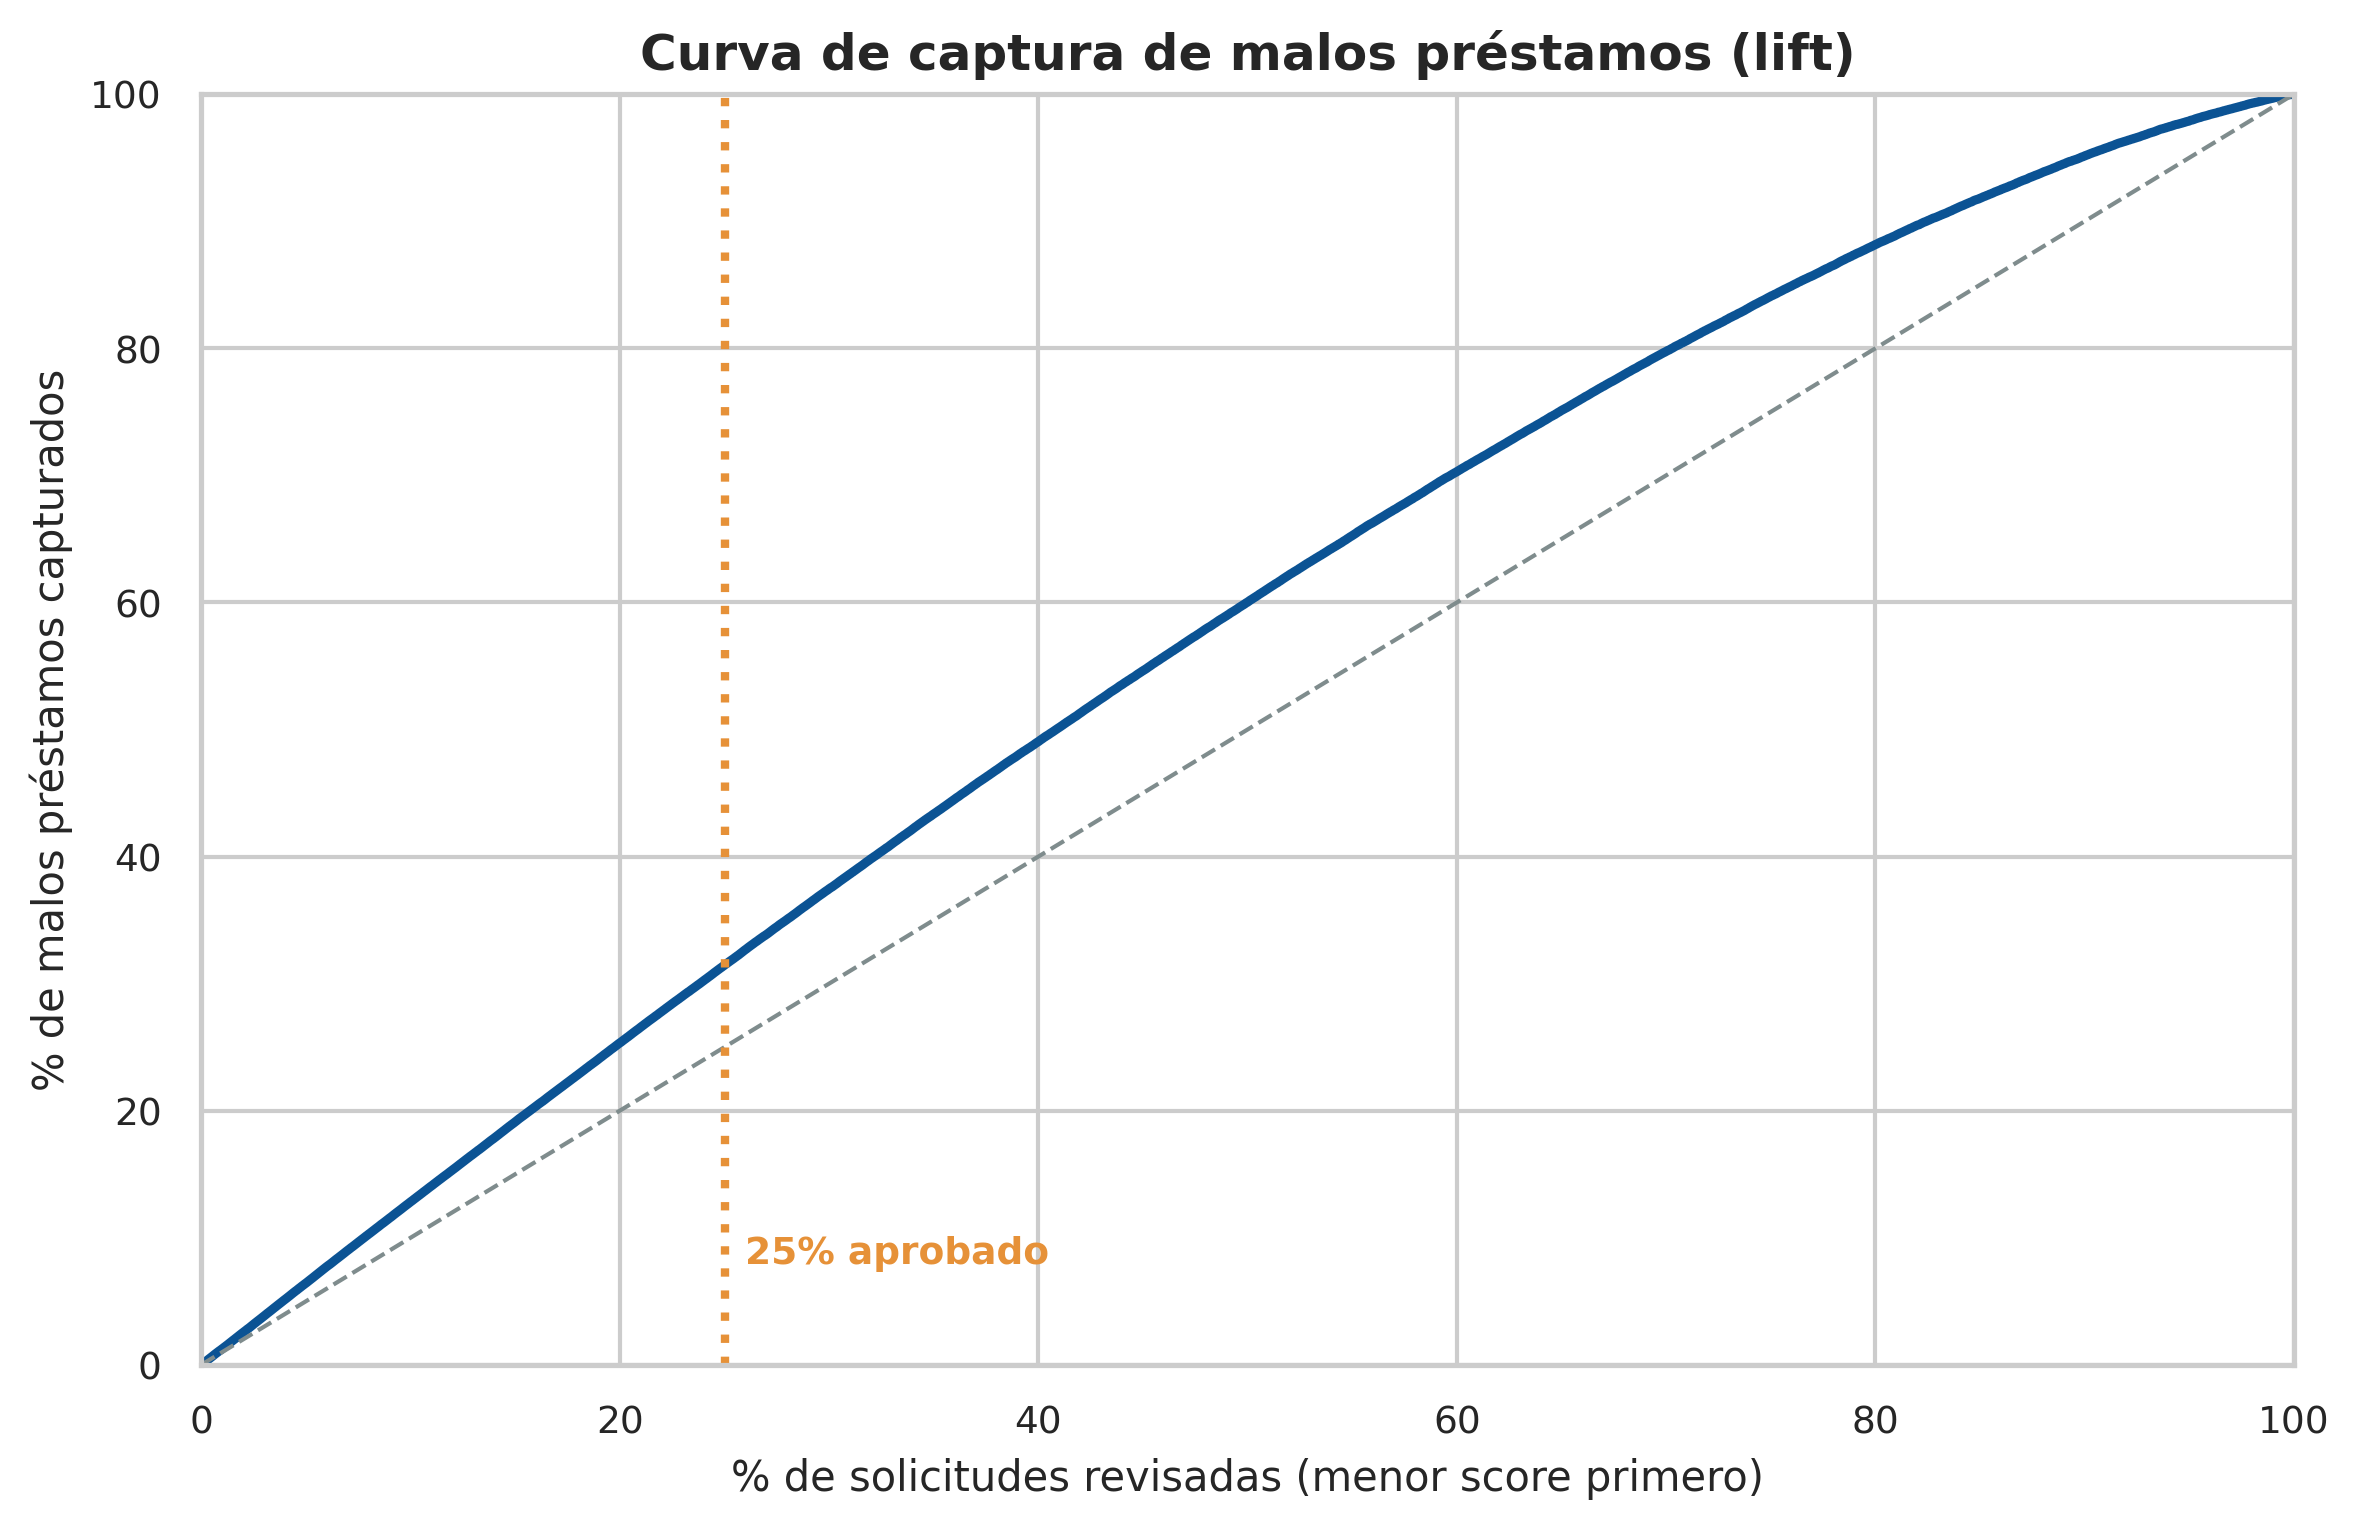
\includegraphics[width=0.72\linewidth]{figuras/model_lift_chart.png}
  \caption{Curva de captura: revisando el 25\% de menor riesgo se excluye
  naturalmente --sin decidir caso a caso-- una proporción alta de los malos.}
  \label{fig:lift}
\end{figure}

\subsection{Sub-segmentación de los aprobados}

La Figura~\ref{fig:seg} compara las tasas de incumplimiento por segmento. El
segmento \emph{Bueno} (37.5\%) presenta una calidad sustancialmente superior
al \emph{Malo} (54.3\%), lo que valida la sub-segmentación como herramienta de
administración de cartera: permite fijar condiciones preferentes al primer
grupo y esquemas de monitoreo intensivo al segundo.

\begin{figure}[H]
  \centering
  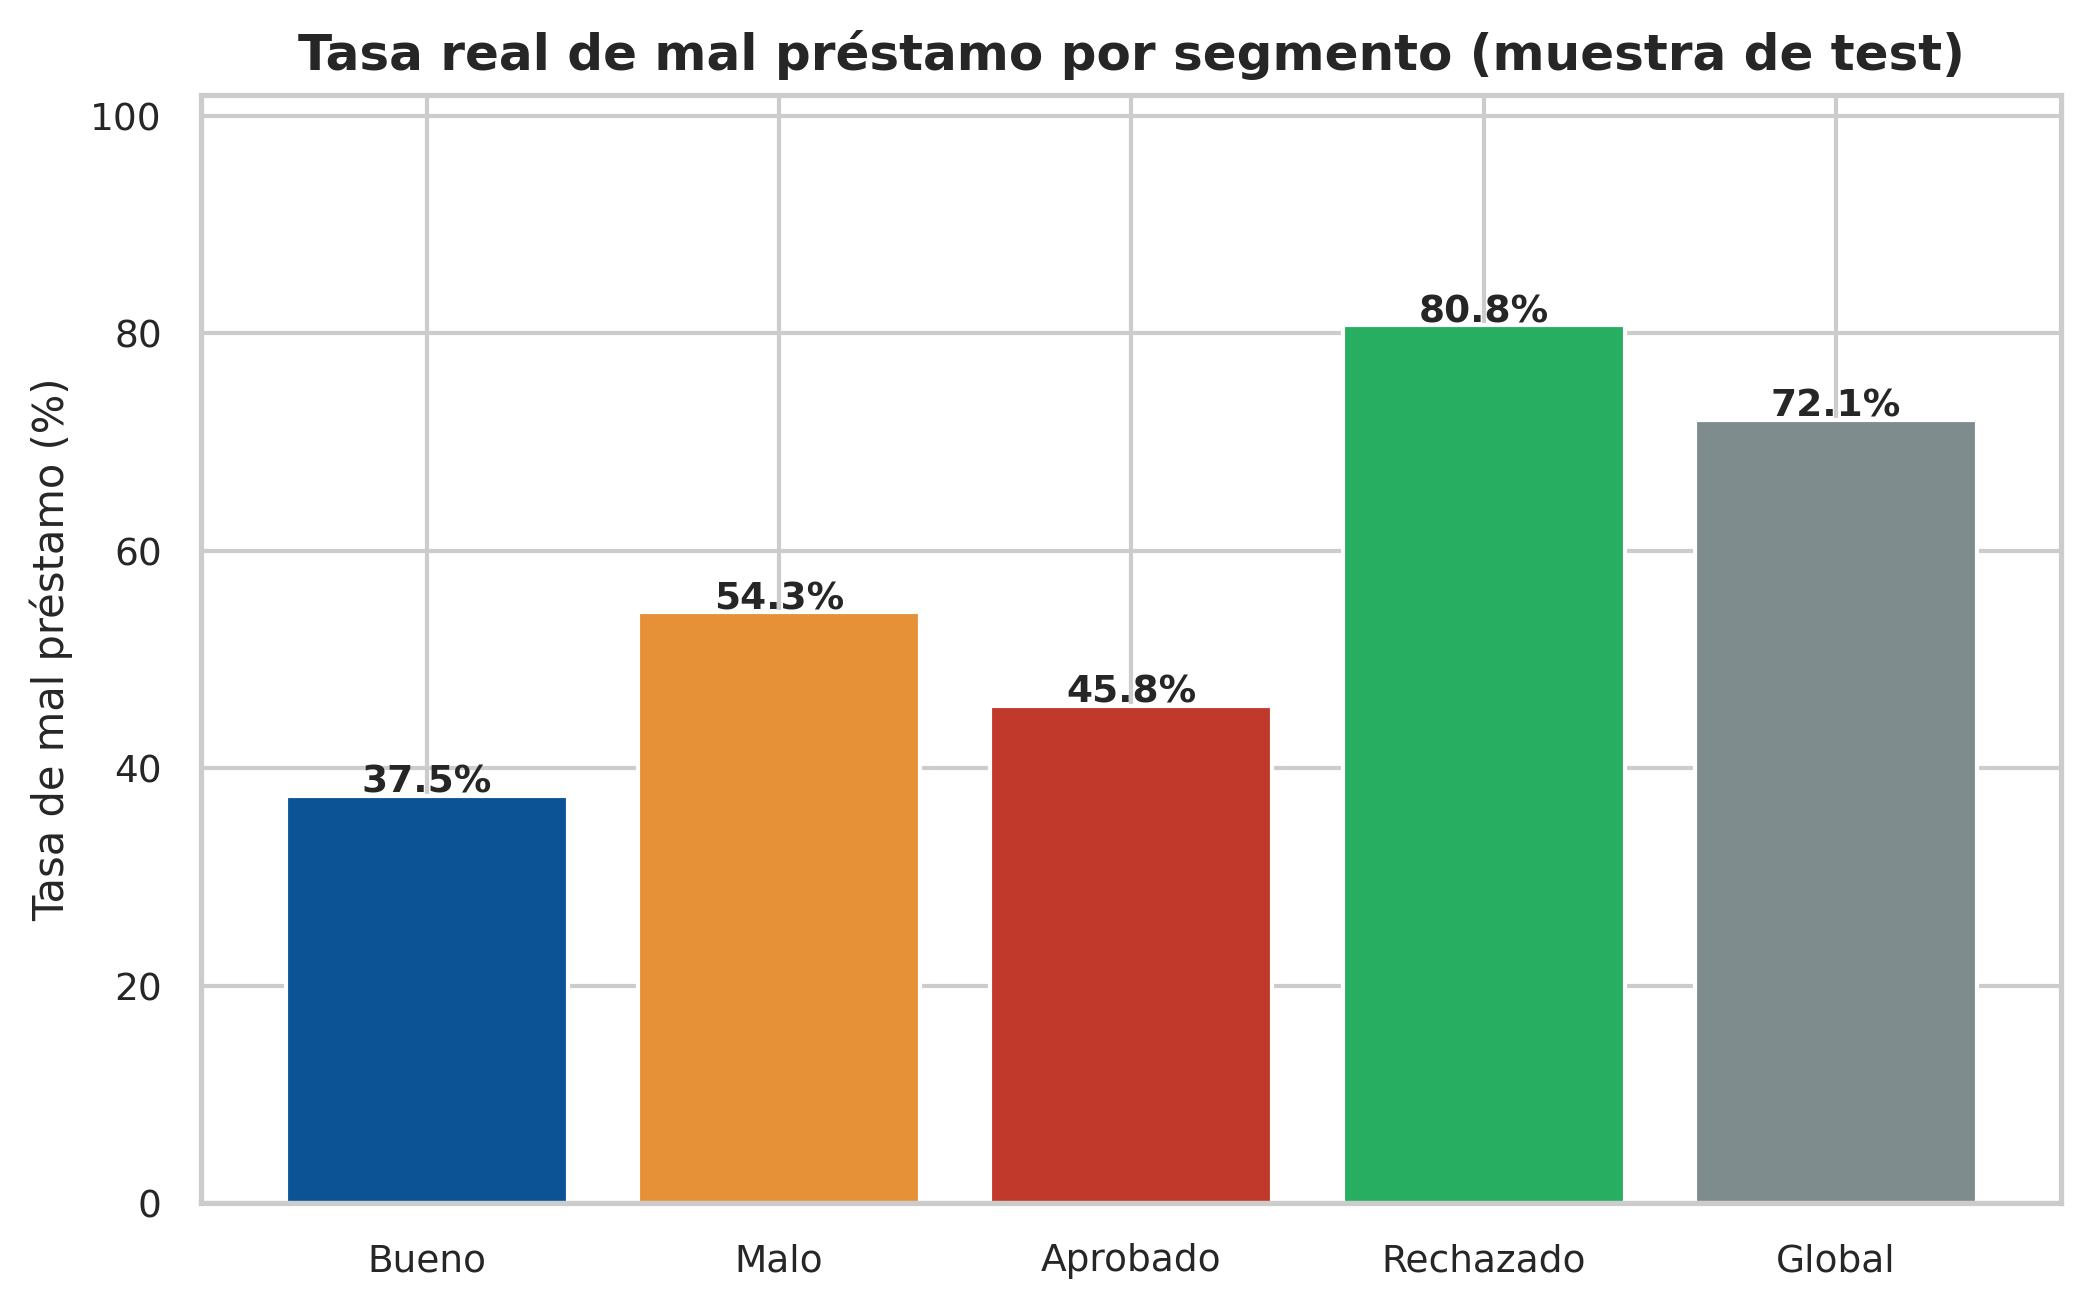
\includegraphics[width=0.78\linewidth]{figuras/model_approval_rates.png}
  \caption{Tasa real de mal préstamo por segmento de la política (test).}
  \label{fig:seg}
\end{figure}

\subsection{Comparación con el modelo de reglas}

La Tabla~\ref{tab:comp} muestra la comparación a igual tasa de aprobación
(25\%).

\begin{table}[H]
  \centering
  \caption{Comparación de métodos a tasa de aprobación de 25\%}
  \label{tab:comp}
  \small
  \begin{tabular}{lccc}
    \toprule
    Método & AUROC & Malos en la cartera aprobada \\
    \midrule
    Regresión logística (test) & \textbf{0.7462} & \textbf{45.8\%} \\
    Reglas del ejercicio (sin recuperación) & 0.5704 & 67.8\% \\
    Reglas del ejercicio (con recuperación) & 0.8538 & 28.6\% \\
    \bottomrule
  \end{tabular}
\end{table}

El modelo estadístico reduce \textbf{un tercio} los incumplimientos de la
cartera frente a las reglas operables (de 67.8\% a 45.8\%), con un AUROC
superior en 0.18. La variante ``con recuperación'' parece superior, pero su
información no está disponible al momento de decidir: sus métricas son
inatendibles y solo se reportan para evidenciar el sesgo del ejercicio
original.

% ----------------------------------------------------------------------
% 6. DISCUSIÓN
% ----------------------------------------------------------------------
\section{Discusión}

\textbf{Sobre el leakage del ejercicio original.} La regla ``recuperación
$\geq 70\%$'' coincide con la definición misma de la variable objetivo: usarla
para decidir es equivalente a leer el resultado del préstamo antes de
otorgarlo. El trabajo revela este sesgo (AUC 0.85 artificial vs.\ 0.57
operable) y propone la corrección metodológica.

\textbf{Sobre la interpretación de la calidad de cartera.} Una tasa de malos
del 45.8\% en la cartera aprobada puede parecer elevada; sin embargo, debe
leerse contra la población (72.1\%): la política casi duplica la calidad de la
cartera y excluye al 84\% de los incumplidos con un costo de originación de
25\%. La definición de \emph{malo} (recuperación inferior al 70\%) es exigente
y agrupa también préstamos con mora parcial, por lo que el nivel absoluto no es
comparable con tasas de \emph{default} regulatorias.

\textbf{Limitaciones.} (i) se utiliza una definición de incumplimiento basada
en recuperación, no en estados regulatorios (\texttt{loan\_status}); (ii) la
base no es una muestra aleatoria del mercado y contiene cohortes de la crisis;
(iii) el scorecard no incorpora restricciones de capital accionario ni
fondeo; (iv) no se realizó análisis de estabilidad temporal por cohortes de
emisión.

% ----------------------------------------------------------------------
% 7. CONCLUSIONES
% ----------------------------------------------------------------------
\section{Conclusiones y trabajo futuro}

Se construyó un \textbf{modelo de decisión crediticia} que cumple la
restricción operativa de aprobar el 25\% de las solicitudes con el menor
riesgo estimado, y que segmenta a los aceptados en \emph{Buenos} y \emph{Malos}
para su administración diferencial. Las conclusiones principales son:

\begin{enumerate}
  \item El scorecard (regresión logística + escala de puntos, corte en 600)
        alcanza \textbf{AUROC 0.746} y \textbf{GINI 0.492} con validación en
        muestra de test sin sobreajuste.
  \item La política aprobó \textbf{24.88\%} de las solicitudes y redujo la
        tasa de malos de la cartera de 72.1\% (población) a \textbf{45.8\%},
        excluyendo al \textbf{84.2\%} de los préstamos incumplidos.
  \item La sub-segmentación separa carteras con 37.5\% y 54.3\% de malos,
        habilitando condiciones preferentes y monitoreo diferenciado.
  \item Frente a las reglas de la práctica original, el modelo estadístico
        reduce un tercio la morosidad de la cartera y detecta y corrige el
        sesgo por leakage.
\end{enumerate}

\textbf{Trabajo futuro:} (i) redefinir el objetivo con estados regulatorios
(\texttt{charge off}) y severidad de pérdida; (ii) validación temporal por
cohortes; (iii) árboles de decisión y \emph{gradient boosting} como modelos
alternativos con \emph{baseline} logístico; (iv) incorporar capital económico
y métricas de rentabilidad (pérdida esperada vs.\ ingreso por interés);
(v) simulación de la estabilidad de los umbrales ante escenarios de estrés.

% ----------------------------------------------------------------------
% REFERENCIAS
% ----------------------------------------------------------------------
\begin{thebibliography}{9}
\raggedright
\small

\bibitem{thomas2002}
L.~Thomas, D.~Edelman y J.~Croxford.
\emph{Credit Scoring and Its Applications}. SIAM Monographs on Mathematical
Modeling and Computation, 2002.

\bibitem{anderson2007}
R.~Anderson.
\emph{The Credit Scoring Toolkit: Theory and Practice for Retail Credit Risk
Management and Decision Automation}. Oxford University Press, 2007.

\bibitem{siddiqi2006}
N.~Siddiqi.
\emph{Credit Risk Scorecards: Developing and Implementing Intelligent Credit
Scoring}. John Wiley \& Sons, 2006.

\bibitem{hanley1982}
J.~A. Hanley y B.~J. McNeil.
``The meaning and use of the area under a receiver operating characteristic
(ROC) curve''. \emph{Radiology}, 143(1):29--36, 1982.

\bibitem{bcbs2005}
Basel Committee on Banking Supervision.
\emph{Studies on the Validation of Internal Rating Systems}. Bank for
International Settlements, Working Paper 14, 2005.

\bibitem{lendingclub}
Lending Club.
\emph{LCDataDictionary}. Base pública de datos de préstamos personales,
disponible en \url{https://www.lendingclub.com}.

\end{thebibliography}

\section*{Reproducibilidad}

Todo el análisis es reproducible con el pipeline \texttt{run\_pipeline.py}
(etapas 00--03) incluido en el repositorio, usando los datos públicos
referidos. Las versiones de las librerías se documentan en
\texttt{requirements.txt}; la semilla aleatoria ($42$) fija la división
train/test.

\end{document}